\documentclass[thesis.tex]{subfiles}
\begin{document}
\chapter{Background and Related Work}
\label{chap:background}

The work presented in this thesis builds on earlier work on policy
languages, in particular work on SecPAL~\cite{becker_secpal:_2006}. In
this chapter we give an overview of earlier work and describe SecPAL
in detail, including its delegation mechanisms. This chapter gives the
background for our work. In \autoref{chap:apppal} we will describe our
changes to SecPAL and how we instantiate it to create a policy
language to describe the policies of the mobile ecosystem.

One approach to designing a policy language is to base it on a logic
of authorization. Authorization logics~\cite{abadi_calculus_1991}
describe rules for deciding when to allow certain actions. A
common use case for these logics is building access control systems. For example, a
user is allowed to read a file if he or she has the proper
permissions. When using authorization logics as policy languages
the policy language describes who can get access to what, but the
authorization logic gives a formal description of how we make that
decision. We want to use authorization policy language to capture the
trust relationships in the mobile ecosystem.

\section{SecPAL}

SecPAL (the \emph{Sec}urity \emph{P}olicy \emph{A}uthorization \emph{L}anguage) is an authorization language developed by Becker, Fournet
and~Gordon to describe policies and delegation chains for distributed
systems~\cite{becker_secpal:_2006}. It is a high-level human-readable
language that separates policy specification and maintenance from the
implementation mechanisms.

SecPAL improves over previous authorization languages in several
ways. It is more expressive than
SPKI/SDSI~\cite{ellison_spki_1999}, and Delegation
Logic~\cite{li_delegation_2003}. It is, arguably, more readable than
XACML~\cite{oasis_extensible_2013} and other XML-based policy
languages.  SecPAL is intuitive and unambiguous with precise proof-theoretic
semantics. Other languages (most notably XACML) have ambiguous
specifications that can be misinterpreted~\cite{ramli_logic_2014}, or
have formal ones retrofitted to the
language~\cite{bryans_reasoning_2005,masi_formalisation_2012}.  In
contrast, Becker~\etal~gives SecPAL's semantics precisely when
describing the language and shows the core language is consistent.

\subsection{Grammar, Evaluation and Semantics}
\label{ssec:grammar-evaluation-semantics}

SecPAL is a language with a simple grammar
(\autoref{fig:secpal-grammar}), three evaluation
rules. (\autoref{fig:secpal-rules}), and an assertion safety condition
(\autoref{fig:assertion-safety}). The language's simplicity makes it
easy to apply to a new domain by instantiating it with predicates and
constraints that describe the domain. For example, to instantiate
SecPAL to describe file access policies we might add predicates like
\texttt{canRead} or \texttt{canWrite} to describe whether a user can
read or write a file. SecPAL's simplicity does not come at the cost of
its expressiveness. SecPAL supports delegation (by using
\emph{can-say} verbs), role and attribute based policies (by using
\emph{can-act-as} verbs) and arbitrary constraints.  SecPAL implements
the idea of principals by allowing them to act as a \emph{speaker} who
\emph{says} assertions about \emph{entities} (who may or may not be
\emph{speakers} themselves). The terms \emph{principal} and
\emph{speaker} are used interchangeably, whereas an \emph{entity} may
denote someone or something that does not or can not make any
assertions themselves.

Delegation lets a principal state that assertions from other
principals can be used in making a decision. Roles allow principals to
state that the subject of an assertion (\autoref{fig:assertion}) is
equivalent to another: effectively aliasing the
subjects to each other.

SecPAL policies are evaluated with respect to an assertion context
\emph{AC}, which holds all known rules and ground facts, and a
delegation level $D$ which either permits or disallows further
delegation. SecPAL evaluation produces an assertion of the form:
\begin{equation*}
 AC, D \models \texttt{{\itshape A} says {\itshape fact}.} 
\end{equation*}
This means that by using that AC, and with delegation either
allowed ($D = \mathtt{inf}$) or not ($D = \mathtt{0}$), SecPAL could show that
$A$ would say the \emph{fact.}

SecPAL assertions can contain variables. A variable can be used in
place of a constant in some parts of an assertion.  The assertion
safety condition (\autoref{fig:assertion-safety}) defines when
variables can be used, and ensures that queries to the policy
terminate when using Becker's evaluation
algorithm~\cite{becker_secpal:_2006}.  To paraphraphrase the rules: a
variable in the head of an assertion is only allowed if it also exists
in the body of the assertion, a variable in the constraint of an
assertion must occur somewhere else (the head or the body), and that
you can't have a conditional fact be a \emph{can-say} statement.  When
evaluating a query against a policy, the \emph{cond}-rule
(\autoref{fig:secpal-rules}) can introduce a renaming $\theta$ that
maps variables to constants in order to resolve the variable against
the query.


\begin{figure}
  \newcommand{\bracetext}[1]{\text{\sffamily #1}}
  \newcommand{\smalltext}[1]{\text{\ttfamily\small #1}}
  \centering
  \begin{equation*}
    \begin{array}{r l}
      \overbrace{\smalltext{`user'}}^{\bracetext{speaker}} & 
                                                             \smalltext{ says }\overbrace{\overbrace{\smalltext{ App }}^{\bracetext{subject}}\overbrace{\smalltext{ isRunnable}}^{\bracetext{predicate}}}^{\bracetext{fact}} \\
                                                           & \overbrace{\smalltext{ if App isFree}}^{\bracetext{condition}}                                                                                                  \\
                                                           & \overbrace{\smalltext{ where hasPermission(App, `INTERNET') = true}}^{\bracetext{constraint}}.
    \end{array}
  \end{equation*}
  \caption{Structure of a SecPAL assertion.}
  \label{fig:assertion}
\end{figure}

\newcommand{\bnfcomment}[1]{\slshape{\sffamily(#1)}}
\newcommand{\secpal}[1]{{\color{BrickRed}\texttt{#1}}}
\begin{figure}\footnotesize\centering\sffamily
  \begin{tabular}{r r l c}
    AC         & $\Coloneqq$ & assertion$_1$ \dots assertion$_n$                           & \bnfcomment{assertion context}     \\
    assertion  & $\Coloneqq$ & e \secpal{says} claim.                                                                           \\
    e          & $\Coloneqq$ & \secpal{X}                                                  & \bnfcomment{variables}             \\
               & $\vert$     & \secpal{'A'}                                                & \bnfcomment{constants}             \\
    predicate  & $\Coloneqq$ & \secpal{has} $\vert$ \secpal{can} $\vert$ \dots             & \bnfcomment{predicates}            \\
    D          & $\Coloneqq$ & \secpal{0}                                                  & \bnfcomment{no further delegation} \\
               & $\vert$     & \secpal{inf}                                                & \bnfcomment{unbounded delegation}  \\
    vp         & $\Coloneqq$ & predicate(\secpal{(}e$_1$\secpal{,} \dots e$_n$\secpal{)})? & \bnfcomment{verb phrase}           \\
               & $\vert$     & \secpal{can-say} D? f                                       & \bnfcomment{delegation of fact}    \\
               & $\vert$     & \secpal{can-act-as}  e                                      & \bnfcomment{role assignment}       \\
    f          & $\Coloneqq$ & e vp                                                        & \bnfcomment{fact}                  \\
    claim      & $\Coloneqq$ & f (\secpal{if} f$_1$,\dots, f$_n$)? (\secpal{where} c)?                                          \\
    c          & $\vert$     & e$^\prime_1 $\secpal{=} e$^\prime_2$                        & \bnfcomment{constraints}           \\
               & $\vert$     & e$^\prime_1 $\secpal{<} e$^\prime_2$                        & \bnfcomment{constraints}           \\
               & $\vert$     & \dots                                                                                            \\
    e$^\prime$ & $\Coloneqq$ & e $\vert$ function(e$_1$,\dots e$_n$)                                                            \\  
               & $\vert$     & \secpal{true} $\vert$ \secpal{false}                        & \bnfcomment{booleans}              \\
               & $\vert$     & integer                                                     & \bnfcomment{numbers}               \\
  \end{tabular}
  \caption[BNF description of SecPAL.]{%
    BNF description of SecPAL as used in this thesis. As originally described by
    Becker, SecPAL is hard to type as it uses subscripts and infinity symbols. We
    replace these with ASCII equivalents, and allow a missing \textsf{D} in the
    \texttt{can-say} statement (equivalent to \texttt{can-say 0}). Terminals are shown
    in {\color{BrickRed} red}.
  }
  \label{fig:secpal-grammar}
\end{figure}

\begin{figure}
  \Fbox{
    \begin{minipage}{1.0\linewidth}\footnotesize
  \newcommand{\avars}[1]{\ensuremath{\text{\itshape vars}\left(#1\right)}}
  \newcommand{\afact}[0]{\ensuremath{\text{\ttfamily\itshape fact}}}
  Let \lstinline{'a' says $\afact$ if $\afact_1\cdots \afact_n$ where $c$.} be an assertion.

  A \textbf{variable} $\mathtt{X} \in \avars{\afact}$ is \emph{safe} if:
  $$\mathtt{X} \in \avars{\afact_1} \cup \cdots \cup \avars{\afact_n}$$

  The \textbf{assertion} \lstinline{'a' says $\afact$ if $\afact_1\cdots \afact_n$ where $c$.} is safe if:
  \begin{enumerate}
  \item
    \begin{enumerate}
    \item If $\afact$ is flat (it is not a can-say fact), all variables in $\avars{\afact}$ are safe.
    \item If $\afact$ is not flat (it is of the form \lstinline{E can-say $~\afact^\prime$}), \texttt{E} is a constant or safe variable.
    \end{enumerate}
  \item $\avars{c}\subseteq\avars{fact}\cup\avars{\afact_1}\cup\cdots\cup\avars{\afact_n}$
  \item $\afact_1\cdots\afact_n$ are all flat.
  \end{enumerate}
\end{minipage}
  }
  \caption{SecPAL's assertion safety conditions.}
  \label{fig:assertion-safety}
\end{figure}

\begin{figure}
  \sffamily
  \footnotesize
  \centering
  \begin{eqnarray*}
    \infer[\textsf{\scriptsize cond}]{%
    AC, D \models A\texttt{~says~}fact\theta
    }{%
    \begin{array}[c]{c}
      \left(a\texttt{~says~}\text{fact}\texttt{~if~}\text{fact}_1,~\ldots,~\text{fact}_k~\texttt{where}~c\right) \in ac \\
      ac,d\models a\texttt{~says~}\text{fact}_i\theta \; \forall i \in \{1\cdots k\}
    \end{array}
    & \models{c\theta}
    & \textsf{vars}(\text{fact}\theta) = \emptyset)
      }                                                                                                                     \\
    \\
    \infer[\textsf{\scriptsize can-say}]{%
    ac, \texttt{inf} \models a\texttt{~says~}\text{fact}
    }{%
    ac, \texttt{inf} \models a\texttt{~says~}b\texttt{~can-say}~d~\text{fact}
    & ac, d \models b\texttt{~says~}\text{fact}
      }                                                                                                                     \\
    \\
    \infer[\textsf{\scriptsize can-act-as}]{%
    ac, d \models a\texttt{~says~}b~\text{verb-phrase}
    }{%
    ac, d \models a\texttt{~says~}b\texttt{~can-act-as~}c
    & ac, d \models a\texttt{~says~}c~\text{verb-phrase}
      }
  \end{eqnarray*}
  \caption[derviation rules used to evaluate {secpal}.]{the derivation rules used to evaluate {secpal}. all {secpal} rules are
  evaluated in the context of a set of other assertions $AC$ as well as an
  allowed level of delegation $D$ which may be \texttt{0} or \texttt{inf}.
  The $\models$ symbol is used by Becker~\cite{becker_secpal:_2006} to describe the derivation rules instead of the more usual $\vdash$.
  This is in order to distinguish SecPAL's derivation rules, from SecPAL's semantic rules (given in \autoref{fig:secpal-semantics}).
}
\label{fig:secpal-rules}
\end{figure}

\begin{figure}\centering\sffamily\footnotesize
  \begin{tabular}{c l p{0.6\linewidth}}
    \toprule
    \multirow{4}{*}{\rotatebox{90}{Concepts}} 
    & $AC,\theta \vdash q$                     
    & Defining relation. A query assertion $q$ is valid given the assertions
      contained in the assertion context $AC$ and a variable substitution $\theta$. \\
    &$\epsilon$                               
    & The empty substitution. \\
    
    \midrule
    \multirow{6}{*}{\rotatebox{90}{Definitions}} &
    1. $AC,\theta \vdash \underbrace{e \text{ says } fact}_q.$ & if $AC,\texttt{inf} \models e\theta \texttt{ says } fact\theta.$\newline and $dom(\theta) \subseteq vars(e \text{ says } fact)$ \\
                                                               & 2. $AC,\theta_1\theta_2 \vdash q_1, q_2$  & if $AC,\theta_1 \vdash q_1$ and $AC,\theta_2 \vdash q_2\theta_1$                    \\
                                                               & 3. $AC,\theta \vdash q_1 \text{ or } q_2$ & if $AC,\theta \vdash q_1$ or $AC,\theta \vdash q_2$                                 \\
                                                               & 4. $AC,\epsilon \vdash \mathsf{not}(q)$   & if $AC,\epsilon \not\vdash q$ and $vars(q) = \emptyset$                             \\
                                                               & 5. $AC,\epsilon \vdash c$                 & if $\models c$                                                                      \\
    \bottomrule                                                                                                                                                                                  \\
  \end{tabular}
  \caption[SecPAL's proof-theoretic semantics.]{SecPAL's proof-theoretic semantics as described by Becker~\cite{becker_secpal:_2006}.}
  \label{fig:secpal-semantics}
\end{figure}

SecPAL's proof-theoretic semantics are given in \autoref{fig:secpal-semantics}.  A
query $q$ to a SecPAL program (which is a collection of facts and
relationships called the \emph{assertion context} or \emph{AC}) asks
if there exists a renaming $\theta$ such that the rules of SecPAL can
derive the possibly renamed query ($AC,\theta \vdash q$
if $AC,\texttt{inf} \models q\theta$)\footnote{$\vdash$ describes if a query
  is valid with respect to an AC, whereas $\models$ says there is a
  valid proof for a SecPAL using the rules of SecPAL.  Conjugation,
  disjunction and negation are allowed within a query, but not when
  evaluating SecPAL.}.  The renaming must only change 
the variables contained in the query. Conjunction and disjunction work
as expected.  Negation is only allowed in an extremely limited form: a
query is false if it has no variables and there is no way
to show that the AC supports the query.  This limited form means that
queries remain decidable: the assertions inside the AC are not permitted to
use negation. 

\begin{figure}
  \centering\footnotesize
  \Fbox{\begin{minipage}{1.0\linewidth}\centering
  \newcommand{\afact}[0]{\ensuremath{\text{\emph{fact}}}}
  \newcommand{\asays}[0]{\ensuremath{\text{\sffamily says}}}
  \newcommand{\avars}[1]{\ensuremath{\text{\itshape vars}\left(#1\right)}}
  $\infer{%
    q~\text{is safe}
  }{%
    \exists O~\text{such that}~\emptyset\Vdash q:O
  }$\vspace{2em}

  $I\Vdash q:O \left\{ \begin{aligned}
      q&\text{~is the query.}\\
      I&\text{~is the set of ground variables before evaluating $q$.}\\
      O&\text{~is the set of newly ground variables after evaluating $q$.}
    \end{aligned} \right.
  $\vspace{2em}
  
  $\infer{%
    I\Vdash e\ \asays\ \afact{} : \avars{e\text{ says } \afact} - I
  }{%
    \afact\ \text{is flat}
  }$\hspace{2em}
  $\infer{%
    I\Vdash c : \emptyset
  }{%
    vars(c) \subseteq I
  }$\hspace{2em}
  $\infer{%
    I\Vdash q_1~\text{\sffamily or }~q_2: O_1 \cap O_2
  }{%
    I\Vdash q_1:O_1 & I\Vdash q_2:O_2
  }$\hspace{2em}
  $\infer{%
    I\Vdash\text{\sffamily not}(q):\emptyset
  }{%
    I\Vdash q:O & \avars{q} \subseteq I
  }$\hspace{2em}
  $\infer{%
    I\Vdash q_1, q_2: O_1 \cup O_2
  }{%
    I\Vdash q_1:O_1 & I\cup O_1 \Vdash q_2:O_2
  }$
  %\hspace{2em}
  %$\infer{%
  %  I\Vdash\exists x(q) : O - \{x\}
  %}{%
  %  I\Vdash q:O & x\not\in I
  %}$
\end{minipage}}
  \caption{SecPAL's IN/OUT query safety condition.}
  \label{fig:safety-conditions}
\end{figure}
 
SecPAL queries are not allowed to contain free variables.
Becker described an \emph{IN/OUT} query safety condition (\autoref{fig:safety-conditions}) that ensured that for any assertion context the set of possible answer substitutions would be finite.
A later extension to SecPAL added guarded universal quantification of varibles, however~\cite{moritz_y_becker_secpal:_2009}. 
The extension allowed queries with a $\forall$ in them, but also required that the query include a \emph{guard}---a statement to restrict the scope of the free variable.
For example, a query to search for all apps (known by Alice) that that were recommended by Bob could be written:
\begin{equation*}
  \forall \mathtt{X}\left( \overbrace{\texttt{Alice says X isApp.}}^{\text{Guard}} \Rightarrow \underbrace{\texttt{Bob says X isRecommended.}}_{\text{Guarded Query}}\right)
\end{equation*}
In this query the \texttt{Alice says X isApp.} is the guard, restricting the scope of \texttt{X} to 
the values that Alice says are apps, and the \texttt{Bob says X isRecommended.} is the guarded query that provides the result.

\subsection{Delegation in SecPAL}
\label{ssec:delegation_in_secpal}

A key feature of SecPAL is the ability to delegate statements. SecPAL was
designed to make access control decisions over large networks. Rather than have
a centralized decision server make all decisions, SecPAL allows
the sharing of information through assertions signed by their speaker. This allows
different principals to take responsibility for different decisions and make
decisions independently. An example of this, expanded from one given by
Becker~\cite{becker_secpal:_2006} and illustrated by us, is of a
researcher attempting to run a query on a cluster using data from a file-server
(\autoref{fig:delegation-example}).

\begin{figure}
  \centering
  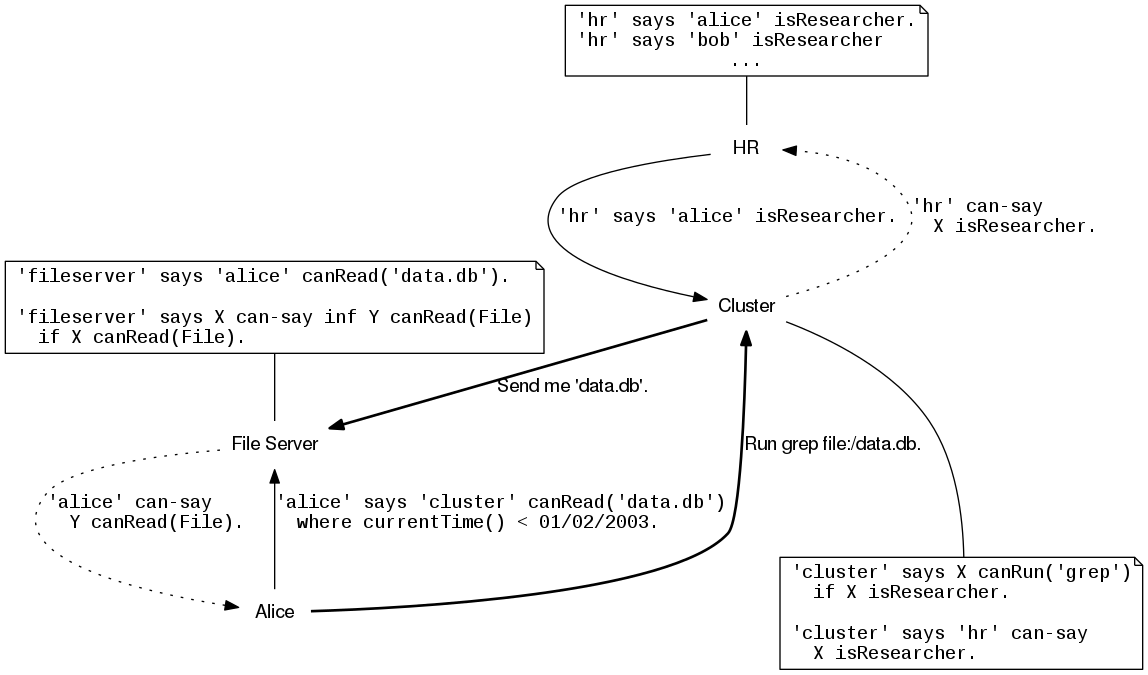
\includegraphics[width=\textwidth]{figures/secpal-example.png}
  \caption[Example of delegation on a cluster.]{Example of delegation when running a command on a cluster.  Bold links show requests, plain links show the sending of SecPAL statements, and dotted links indicate delegation relationships.  SecPAL assertions at each location are shown in notes.}
  \label{fig:delegation-example}
\end{figure}

Alice requests the cluster run a search on her data.  Her data is on the file-server.
The cluster has a SecPAL policy that only researchers can run the search.
It also has a rule that says the human resources department (HR) can say who is a researcher.
\begin{lstlisting}
'cluster' says X canRun('grep')
  if X isResearcher.

'cluster' says 'hr' can-say
  X isResearcher.
\end{lstlisting}
The cluster queries HR if Alice is a researcher. HR responds by saying she is.
\begin{lstlisting}
'hr' says 'alice' isResearcher.
\end{lstlisting}
The cluster does not know how HR knows that Alice is a researcher. But it
is content \emph{to trust} HR's assertion that she is.  HR may have a SecPAL
instance and policy of their own to make this decision and send it to the
cluster. Alternatively they might be using a conventional database.  Provided
they give this SecPAL assertion to the cluster, it does not care
how they came by it.  The one limitation the cluster has is that it
\emph{must} be HR telling them. HR cannot delegate the decision
further.

The cluster is now convinced that Alice may run the search.
It requests the database from the file server.  The file
server knows that Alice can read her data and that anyone who can read
a file may say who else can read it.
\begin{lstlisting}
'fileserver' says 'alice' canRead('data.db').
'fileserver' says X can-say inf Y canRead(File)
  if X canRead(File).
\end{lstlisting}
Using SecPAL, the file server determines that Alice can say who
reads her data.  Alice gives the file server a statement that
the cluster can read her file (for a short time
period).
\begin{lstlisting}
'alice' says 'cluster' canRead('data.db')
  where currentTime() < 01/02/2003.
\end{lstlisting}
The file server gives the cluster the data.
The cluster runs the search and hands the results back to Alice.

\begin{figure}
  \centering
  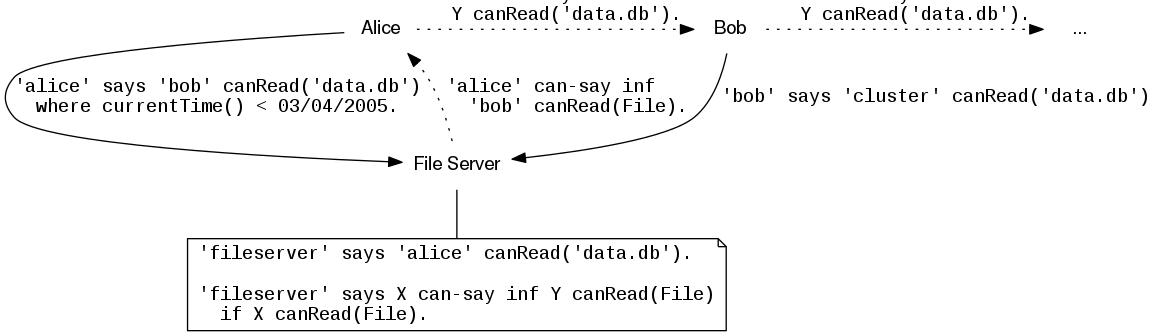
\includegraphics[width=\textwidth]{figures/secpal-example-delegation.png}
  \caption{Example of unbounded delegation.}
  \label{fig:unbounded-example}
\end{figure}

This simple example shows how different principals can make decisions using delegation mechanisms.
SecPAL allows for more complicated delegation relationships, however. 
The file server gave Alice the ability to delegate who could read her file by using the \texttt{can-say inf} verb.
Alice might allow Bob to share her data set with others who might also be allowed to share it for a limited time (\autoref{fig:unbounded-example}).

\begin{figure}
  \centering
  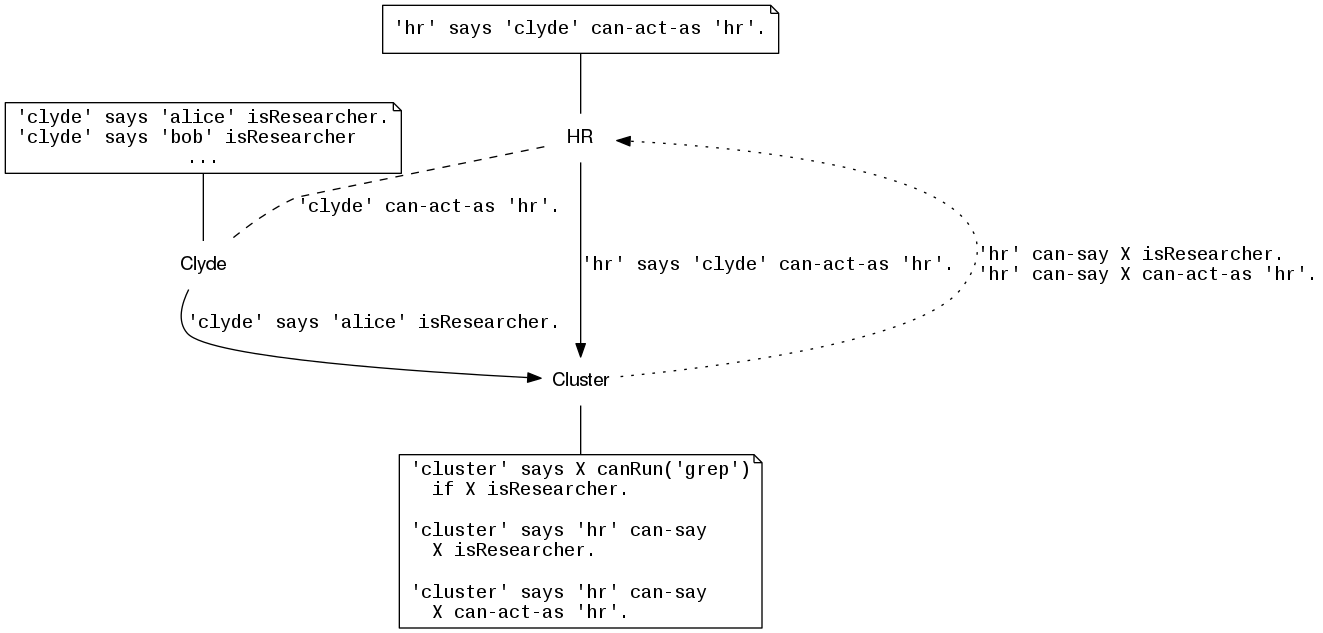
\includegraphics[width=\textwidth]{figures/secpal-example-roles.png}
  \caption[Example of delegation with roles.]{Example of delegation with roles.  Role relationships are shown with dashed links.}
  \label{fig:roles-example}
\end{figure}

An alternative to asking to the HR server directly if Alice is a
researcher is to use roles (shown in
\autoref{fig:roles-example}). Many people work in HR. The cluster
might accept the word of any of the people who work there. To do this
the cluster delegates to HR to name anyone who \emph{acts as}
HR. Suppose that HR responds that Clyde can act for them.
\begin{lstlisting}
'cluster' says 'hr' can-say
  X can-act-as 'hr'.

'hr' says 'clyde' can-act-as 'hr'.
\end{lstlisting} Now, on the cluster, Clyde's word is as good as HR's. Clyde
sends the necessary facts about Alice. The policy check now runs as before. Note
that the restrictions on HR also apply to Clyde: he still cannot delegate the
decision further. Clyde may have more capabilities than HR if there are other
provable assertions about him. The \emph{can-act-as} means that Clydes is at
least as powerful as HR: he inherits HR's capabilities.

\begin{figure}
  \centering
  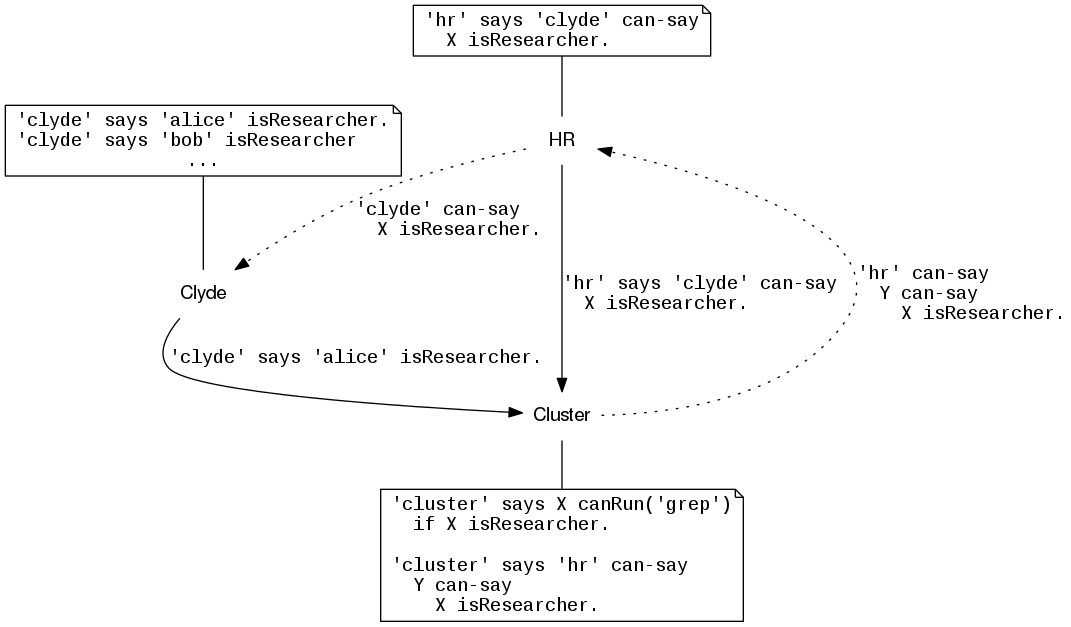
\includegraphics[width=\textwidth]{figures/secpal-example-delegation2.png}
  \caption{Example of depth-bounded delegation.}
  \label{fig:depth-example}
\end{figure}

Depth-bounded delegation with the \emph{can-say} statement is an alternative to
roles (\autoref{fig:depth-example}). Instead of letting HR state who is a
researcher to HR, the cluster lets HR \emph{decide who decides}. HR delegates to
Clyde and the process continues as before. Depth-bounded delegation allows
delegation statements to be chained to an arbitrary (but finite) depth, without
allowing for unbounded delegation (as shown in \autoref{fig:unbounded-example}). It is preferable to roles as it allows HR to
delegate some but not all decisions to others. If role assignment is used then,
on the cluster, anywhere \texttt{'hr'} follows the \texttt{says} in an
assertion, then it can be replaced with \texttt{'clyde'}: they are the same.

SecPAL's delegation mechanisms can describe many trust relationships
between entities, as we have described above. Yet it remains
conceptually and semantically simple, by using just the \texttt{can-say} and \texttt{can-act-as} phrases to capture them. This power makes SecPAL
attractive for situations where entities are distributed and there is
no central decision point, as we can capture the trust relationships
between entities and at different places. This makes SecPAL a very
appropriate language to model the policies of the mobile ecosystem, as
every device, user, company and store has their own policies and makes
their own decisions, sometimes by talking to each other. We will
discuss our reasons for using SecPAL to capture the policies of the
mobile ecosystem further in \autoref{chap:apppal}, but to sumarise its
ability to delegate and capture policies makes it a good starting
point.

\subsection{Integrating SecPAL}

Becker's description of SecPAL does not give details as to how a system using
SecPAL should be implemented. For example, if SecPAL were to be used to add
access controls to an email system, the language itself does not describe when
the mail server should check the policy to see if a user can access their mail.
We might imagine that a user authenticates with mail~server using LDAP, and then
before allowing them access to their mail, queries a SecPAL policy (where
\lstinline!'user'! has been replaced by the real user):
\begin{lstlisting}
'it-admin' says 'user' canReadMailOf('user').
\end{lstlisting}
SecPAL does not, however, describe how or when the query should be made, only
how to process it when it has been. The decisions as to how and when are left to
the person implementing the system.

Similarly, If a policy query uses delegation then the assertion context being queried must
contain the necessary facts from the delegated parties before checking the
query. SecPAL doesn't say when or how these statements should be fetched, just
what to do with them once they have been. Later languages, such as
DKAL~\cite{gurevich_dkal:_2008}, give explicit protocols to enable information
sharing; but for SecPAL the decision of how to implement and automate these
procedures is left to the system designers.


\section{Policy Languages}
\begin{figure}
  \centering\sffamily\scriptsize
  \begin{chronology}[5]{1987}{2017}{\textwidth}
    \event{1988}{X.509}
    \event{1991}{A Calculus for Access Control~\cite{abadi_calculus_1991}}
    \event{1994}{Authentication in the Taos OS~\cite{wobber_authentication_1994}}
    \event{1996}{PolicyMaker~\cite{blaze_decentralized_1996}}
    \event{1998}{KeyNote~\cite{blaze_keynote:_1998}}
    \event{1999}{SPKI/SDSI\cite{ellison_spki_1999}}
    \event{2000}{Delegation Logic~\cite{li_practically_2000}}
    \event{2001}{Ponder~\cite{damianou_ponder_2001}, XACML}
    \event{2002}{RT~\cite{li_design_2002}, Binder~\cite{detreville_binder_2002}}
    \event{2004}{Cassandra~\cite{becker_cassandra:_2004}}
    \event{2005}{XACML 2.0}
    \event{2006}{SecPAL~\cite{becker_secpal:_2006}}
    \event{2008}{DKAL~\cite{gurevich_dkal:_2008}}
    \event{2009}{DKAL2~\cite{yuri_gurevich_dkal2---simplified_2009}, Ponder2~\cite{twidle_ponder2:_2009}, SecPAL4P~\cite{becker_framework_2009}}
    \event{2010}{XACML 3.0~\cite{oasis_extensible_2013}}
    \event{2011}{SecPAL4DSA~\cite{aziz_secpal4dsa:_2011}}
    \event{2013}{DKAL$\star$~\cite{jeannin_dkal*:_2013}}
    \event{2016}{AppPAL~\cite{hallett_apppal_2016}}
  \end{chronology}
  \caption{Timeline of the development of different policy languages.}
  \label{fig:policy-language-chronology}
\end{figure}


We have introduced SecPAL to describe policies, and will study it further in the
rest of the thesis to describe the policies of the mobile ecosystem. In this
section we give a survey of some other influential policy languages. A timeline
of the development of the languages mentioned here is shown in
\autoref{fig:policy-language-chronology}.

\paragraph*{PolicyMaker.}  PolicyMaker~\cite{blaze_decentralized_1996}
is a language for permitted actions.  It grew out of the logics of
authentication of Wobber, Abadi, Burrows and
Lampson~\cite{wobber_authentication_1994,abadi_calculus_1991}; as well
as a dissatisfaction with identification mechanisms such as X.509 and
PGP certificates. These mechanisms identified users but could not link
them to what they could do.

To describe the authorizations, assertions hold trust information.
Many assertions form a policy. An assertion has a source (either the
local policy document or a public key). The source \emph{asserts} that
the holder of a key (or more complex arrangements such as three of
four keys) can do any action that matches the \emph{filter}. The
filter itself is an arbitrary program that can make a yes/no decision.
Blaze~\etal~give examples using regular expressions and a reduced
version of AWK~\cite{aho_awk-pattern_1979}. They note, however, that
any programming language could be used. The device policy can be
queried by a key holder \emph{requesting} a given action. 

To integrate PolicyMaker into a real system, software would have to be modified
to automatically send PolicyMaker queries to a central query server in response
to events, in order to decide what to do next.
% 
Blaze~\etal~give an example of this scheme being used as part of an
email server. A user, Alice, identified by key \texttt{0x12345678} can
send emails with the \texttt{from} header set to Alice and the
organization set to Bob Labs.

PolicyMaker is installed on a server. It receives queries and gives answers.
The policy installed on the server in this example would be:

\begin{lstlisting}
policy ASSERTS
  pgp:'0x12345678'
  WHERE PREDICATE=regexp:'(From: Alice) &&
    (Organization: Bob Labs)';
\end{lstlisting}

When Alice sends an email using a PolicyMaker enhanced SMTP
client she signs her message with her key.  The mail server
checks the signature and queries the policy server with her message:

\begin{lstlisting}
  pgp:'0x12345678'
  REQUESTS  'From: Alice
             Organization: Bob Labs

             Hello World!';
\end{lstlisting}

If Alice's message is okay, then the SMTP server will send it.  If it does not
match the policy, then it will not.

\paragraph*{KeyNote.}
PolicyMaker is the basis for KeyNote~\cite{blaze_role_1999,blaze_keynote:_1998}.
KeyNote simplifies the arbitrary filter languages, offering instead one based on
C that always returns a boolean answer. KeyNote allows the policy server to do
the signature verification instead of the querying application. It also makes the
syntax more readable. KeyNote also trades PolicyMaker's generality for a more
realistic scenario using public-key infrastructure. The prior policy for KeyNote
could be written:

\noindent\begin{minipage}{\textwidth}
\begin{lstlisting}
Authorizer: "POLICY"
Licensees: "RSA:abc123"

KeyNote-Version: "2"
Local-Constants: Alice="RSA:12345678" 
Authorizer: "RSA:abc123"
Conditions: (app_domain == "RFC822-EMAIL") &&
    (name="Alice") &&
    (organization="Bob Labs");
\end{lstlisting}
\end{minipage}

As with PolicyMaker, the integration of KeyNote into any application is left to
developers.  Consequently the automation of any queries (and deciding what to do
with whatever results KeyNote may return) is left to the application.
Blaze~\etal{} note that~\cite{blaze_keynote_1999}:

\begin{quotation}``KeyNote does not directly enforce policy it only provides advice
to the applications that call it. In other words, KeyNote assumes that the
application itself is trusted and that the policy assertions it specifies are
correct. Nothing prevents an application from submitting misleading or incorrect
assertions to KeyNote or from ignoring KeyNote altogether.''
\end{quotation}

Checking whether a PolicyMaker or KeyNote policy is satisfied is
NP-hard~\cite{blaze_compliance_1998}. PolicyMaker assertions can involve
arbitrary programs written in Turing complete languages. Blaze~\etal{} restrict
these programs to those that run in polynomial time for all inputs pertinent to
a request.

A weakness of these languages is that they cannot express relationships among
users. You cannot have policy where the subject is a set of users. The example
policy could not be written as \emph{anyone working in R\&D can send email from
Bob Labs.}

%\subsection{SPKI/SDSI}

\paragraph*{SPKI/SDSI.}
Unlike PolicyMaker, SPKI/SDSI~\cite{ellison_spki_1999} was
designed to associate keys with roles.  A user, Alice with key~$K_A$,
can present a certificate that says she \textbf{can act as} (a role assignment) a \emph{Bob Labs
employee} (authorized by Bob with key~$K_B$) for one~year.

\noindent\framebox[\textwidth]{\small
\(
  (K_A,~\text{\tt BobLabsEmployee},~K_B,~1~\text{year})
\)%
}

Bob can also create authorization certificates to let his employees
to send emails. Optionally they can delegate the decision further.

\noindent\framebox[\textwidth]{\small
\(
 (K_B,~(K_B,~\text{\tt BobLabsEmployee}),~\bot,~\text{\ttfamily send\_email},~1~\text{year})
\)%
}

PolicyMaker checks whether to allow a specific user's action. SPKI/SDSI associates users with roles and
roles with tasks. The SPKI/SDSI version of the email sending policy (shown above) does not
specify that all emails sent by Employees must have a field listing the lab as
the sending organization. That part of the policy must be added by
whatever implements the \texttt{send\_email} functionality. One of the
advantages of SPKI/SDSI is that it allows a higher-level view of the policy by
associating groups of users with a role, and roles with allowed actions, rather than specifying the precise mechanism of the checks.

SPKI/SDSI does not have a formal semantics.  The language's precise
meaning must be inferred from RFC 2693, which loosely defines it in
English~\cite{ellison_spki_1999}. There are several later attempts at
fitting semantics to the
language~\cite{joseph_y._halpern_logic_1999,abadi_sdsis_1998,howell_formal_2000,dwaine_clarke_certificate_2001}.
Not all covered every aspect of SPKI/SDSI's features, however. No
definitive standard has appeared.

\paragraph*{RT.}
The focus on roles led to the RT family of
languages~\cite{ninghui_li_design_2002}. RT associates policy
decisions with roles. This is similar to how \ac{RBAC} systems associate access
decisions to the roles a user holds.  Policies are expressed as Horn
clauses.  A rule such as:

\begin{lstlisting}[language=prolog]
Bob.employee :- alice.
Bob.employee.sendEmail :- Bob.employee.
\end{lstlisting}

\noindent is read as \emph{Bob says Alice is an employee, and Bob says
an employee can send emails if they are an employee.}  Li~\etal{}
describe many variants of RT with various features.  The most basic
variant is \RT{0}{}~\cite{li_distributed_2003}. \RT{1}{} adds support
for parameterized roles. \RT{2}{} adds logical objects on top of the
roles.  As well as these variants, the RT family of languages supports
optional feature sets: \RT{}{T} allows for policies with thresholds
(i.e. Alice can email someone if two out of three of the board members
of her company approve it). \RT{}{C} adds constraints. Finally,
\RT{}{D} adds delegation~\cite{ninghui_li_design_2002}.

Unlike PolicyMaker, the RT family of languages is tractable. Li~\etal~prove a
guarantee that a query will be answered soundly in polynomial time in the size
of the policy. To give this guarantee, the researchers showed the languages
could be reduced to Datalog. Datalog is a database language with known
complexity guarantees and fast evaluation. Datalog is similar Prolog, but
without negation, complex arguments, and the \texttt{is} statement. They also
showed similar languages, like Binder~\cite{detreville_binder_2002} and
Delegation~Logic~\cite{li_delegation_2003,li_practically_2000}, could be
described using Datalog as well.

Datalog is limited in that it cannot describe structured data. Consider a rule
that lets Alice send email between 9am and 5pm. We might want some function to
compare whether a time is within a range. In Datalog we cannot trivially write
this function. We would have to say for each possible time if it is in that
period. Generally, when there is data that has structure such as file paths,
times or numeric intervals: Datalog databases can become overly large.

To solve this Li~\etal{}~modified Datalog to create
Datalog\textsuperscript{C}~\cite{li_datalog_2003}. Datalog\textsuperscript{C}
is based on Constraint
Datalog~\cite{revesz_constraint_1995,revesz_safe_1998} and supports
constraints whilst keeping Datalog's tractability. It focuses on the
constraints typical to a policy languages (such as constraints for
handling files and directories) instead of those for database
programming.

Showing a policy language is translatable to Datalog\textsuperscript{C} allows
the language author to prove that evaluating policies in their language can be
done with the same time and space complexities as Datalog\textsuperscript{C}.
Datalog\textsuperscript{C} is used as a foundation for many other policy
languages including SecPAL as well as RT.

\paragraph*{Ponder.}
Ponder, like SecPAL, is a language for specifying policies for distributed
systems~\cite{damianou_ponder_2001}. Ponder supports positive and negative
authorization, delegation, obligation, roles and constraints. It uses
constraints to extract the attributes of principals, read state, and deal with
time. A policy that trainee engineers are not allowed to send emails could be
written:

\begin{lstlisting}
inst auth- engineersCanEmail {
  subject e =/Engineer;
  target  /mail_server;
  action send_email();
  when e.status() == ``trainee'';
}
\end{lstlisting}

Since Ponder allows positive and negative policies, conflicts can occur. Ponder
does not resolve the conflicts itself. Instead, it detects them using static
analysis and reports them to the policy author as bugs in the policy
specification. Ponder2~\cite{twidle_ponder2:_2009} simplified Ponder and added
policies for decentralized environments. 

Ponder2 also provides a control language called \emph{PonderTalk}, which lets
the decision engine send messages to the objects it manages, as well as the
objects send messages between themselves. This allows for the automation of some
queries in response to PonderTalk message being sent, as well as the management
of obligations by allowing different objects to notify others of what they
\emph{must} do.


\paragraph*{Cassandra.}
Cassandra is a trust management language to model large systems.
It was demonstrated on the NHS Spine: a system to let healthcare
workers share patient
data~\cite{becker_cassandra:_2004,becker_cassandra:_2004-1}.  The
language is similar to RT, using both a Datalog\textsuperscript{C} and some
of its syntax. Cassandra, however, focuses on roles instead of general access
control mechanisms.  Principals \emph{activate} roles when they need to act in its
capacity.  This lets one principal hold different roles, with
different capabilities, at different times and at different
locations.  A \emph{hospital} \emph{admin} might allow a
\emph{clinician} access to a \emph{patient}'s records if they
have the role of \emph{Clinician} at the hospital, and can
\emph{activate} the role of \emph{Treating Clinician} for that patient
at this \emph{hospital}:

\noindent\begin{minipage}{\textwidth}
\begin{lstlisting}
hospital@admin.permits(clinician, Read-Records(patient)) <-
  hospital@hasActivated(clinician, Clinician(hospital)),
  hospital@canActivate(clinician, TreatingClinician(hospital, patient))
\end{lstlisting}
\end{minipage}

A prototype of Cassandra was implemented allowing it to answer some of the queries
associated with requesting electronic health records, but this wasn't further
developed (that we know of) into an automated system for supplying health records.

Cassandra allows for powerful control of different roles, and enables
delegation by allowing third-parties to activate and remove roles
on others.  
Becker worked on Cassandra for his doctorate.  He went on to work on SecPAL.

\paragraph*{DKAL}
The DKAL family of
languages~\cite{jeannin_dkal*:_2013,gurevich_dkal:_2008,yuri_gurevich_dkal2---simplified_2009}
grew from SecPAL as a policy language for a distributed system's
interacting agents~\cite{blass_introduction_2012}. Assertions are
communicated as signed statements called \emph{infons} between
principals. For example Alice might wish to recommend Bob an
app. Alice, therefore, sends to Bob the infon:

\begin{lstlisting}
alice said com.rovio.angrybirds is a good app.
\end{lstlisting}

Bob is free to do with this information as he wishes. He might accept
app recommendations from anyone and may have a rule to learn facts:

\noindent\begin{minipage}{\textwidth}
\begin{lstlisting}
with M: String, P: Principal
  upon
    P said M is a good app
  do
    learn P said M is a good app
\end{lstlisting}
\end{minipage}

DKAL2~\cite{yuri_gurevich_dkal2---simplified_2009} simplifies DKAL
language removing SecPAL's constructs for roles (the \emph{can-act-as} statement)
as the authors of DKAL and DKAL2 could not find a use for them in practice.  It also adds
support for sending infons if the recipient has completed an action:
for example only sending an app recommendation if the recipient has
asked for it.
DKAL\textsuperscript{$\star$}~\cite{jeannin_dkal*:_2013} took the ideas of information sharing
further and showed how to create executable protocols from DKAL programs.

DKAL improves over SecPAL by giving a means for transferring and
reacting to information. These might be helpful to describe how
protocols worked within the mobile ecosystem and for expanding how
obligation policies would be triggered.  The authors of DKAL showed
that all SecPAL policies could be expressed in
DKAL~\cite{gurevich_dkal:_2008}. 

The work on AppPAL in this thesis is based on SecPAL rather than a DKAL-based language. 
As DKAL extends SecPAL, and is backwards compatible with SecPAL, AppPAL could gain, if needed,
increased expressiveness and the ability to describe protocols just by switching interpreters.
For the work described in this thesis however, we did not require the additional expensiveness.

\paragraph*{SecPAL Extensions.}
We started this chapter, by describing SecPAL. Since SecPAL was first described
various tweaks and extensions were made to the language. SecPAL was extended to
allow existential queries. This allowed it to answer
queries such as \emph{``does Alice say Bob can read any of her files?''} or
\emph{``do all Alice's apps meet her installation policy?''}, which could only
be answered by manually making multiple queries before. 
%
Becker also described the possibility of dynamic assertion retrieval, which
would allow SecPAL to fetch and add assertions to its assertion context when
making queries. In the case of delegation this would allow a delegated
principals assertions to be imported dynamically rather than having to be
present in the AC before evaluating a query. Becker defined a safety condition,
but didn't describe a protocol for retrieving assertions,
however~\cite{moritz_y_becker_secpal:_2009}.

Becker also noted that roles and the \emph{can-act-as} statement had proven to
be of limited use. Delegation using \emph{can-say} could replace it with greater
control in all cases Wherever that \emph{can-act-as} to use exclusively depth
bounded delegation (as we showed in \autoref{ssec:delegation_in_secpal}). 

\paragraph*{XACML}

XACML is a policy language with an industrial
standard~\cite{oasis_extensible_2013} that can be extended to fit many
scenarios. It is an attribute based policy language, but can also describe
role-based policies. It has tooling and enforcement infrastructure available
from Oracle.  The third version of the language (which supports delegation) was
released just after we started our own work on AppPAL.
%
As a standard, it is important to summarize and briefly describe
why we chose to base our own work on SecPAL, a comparatively obscure policy
language, instead of the more well-known XACML.

XACML policies are expressed as sets of \emph{rules} that describe whether a
specific action should be allowed or denied. When making a \emph{request} if a
rule's target matches it then the appropriate action should be taken. Rules are
combined into policies containing many rules which can contradict each other if
multiple ones match a given request. To handle contradictions a \emph{combining
algorithm} is used to decide how to proceed. Typical algorithms include:

\begin{description}
  \item[Permit-overrides.] If a rule gives a \emph{permit} result, then the request is permitted.
  \item[Deny-overrides.] If a rule gives a \emph{deny} result, then the request is denied.
  \item[First-applicable.] The rules have an order of precedence. The first rule that gives a result decides the outcome.
  \item[Only-one-applicable.] Only one rule may match. If there are multiple matches, then an error is returned.
\end{description}

XACML's designers used natural language to describe the semantics of XACML. This
makes the semantics notoriously difficult to
interpret~\cite{ramli_detecting_2015}. There have been several attempts to
describe XACML's semantics
formally~\cite{ramli_xacml_2012,ramli_logic_2014,bryans_reasoning_2005}. Some of
these translations only describe a subset of XACML's
syntax~\cite{halpern_using_2008}. Others describe older versions of XACML which
are not compatible with the latest language versions~\cite{ahn_reasoning_2010},
Others have been found to contain mistakes caused by ambiguities in the
XACML specification~\cite{bruns_access-control_2008,halpern_using_2008}. All
these attempts help us understand XACML, but the lack of a single standard
semantics make it less attractive to extend to a new domain. As the language
grows and changes there are no present guarantees that any of the formal
semantics will remain correct and applicable to the current version of XACML. In
contrast, SecPAL's semantics are given precisely by
Becker~\cite{becker_secpal:_2006}.

Whilst SecPAL was designed for readability, XACML policies are verbose and
difficult to read. For example, to describe a simple policy that grants a principal,
\emph{Alice}, permission to do whatever she wants we might write:

\noindent\begin{minipage}{\linewidth}
\begin{lstlisting}
<xacml3:Policy xmlns:xacml3="urn:oasis:names:tc:xacml:3.0:core:schema:wd-17"
  PolicyId="http://axiomatics.com/alfa/identifier/alice.policy"
  RuleCombiningAlgId="urn:oasis:names:tc:xacml:3.0:rule-combining-algorithm:permit-overrides"
  Version="1.0">
  <xacml3:Description />
  <xacml3:PolicyDefaults>
    <xacml3:XPathVersion>http://www.w3.org/TR/1999/REC-xpath-19991116</xacml3:XPathVersion>
  </xacml3:PolicyDefaults>
  <xacml3:Target>
    <xacml3:AnyOf>
      <xacml3:AllOf>
        <xacml3:Match MatchId="urn:oasis:names:tc:xacml:1.0:function:string-equal">
          <xacml3:AttributeValue
            DataType="http://www.w3.org/2001/XMLSchema#string">alice</xacml3:AttributeValue>
          <xacml3:AttributeDesignator 
            AttributeId="urn:oasis:names:tc:xacml:1.0:subject:subject-id"
            DataType="http://www.w3.org/2001/XMLSchema#string"
            Category="urn:oasis:names:tc:xacml:1.0:subject-category:access-subject"
            MustBePresent="false"
          />
        </xacml3:Match>
      </xacml3:AllOf>
    </xacml3:AnyOf>
  </xacml3:Target>
  <xacml3:Rule 
      Effect="Permit"
      RuleId="http://axiomatics.com/alfa/identifier/alice.policy.Id_18">
    <xacml3:Description />
    <xacml3:Target />
  </xacml3:Rule>
</xacml3:Policy>
\end{lstlisting}
\end{minipage}

To help developers write policies, alternative notations are available that
compile into XACML's XML notation. ALFA is an alternate notation for
XACML~\cite{oasis_xacml_technical_comitee_abbreviated_2015} maintained by the
XACML developers. The equivalent ALFA policy of the above \emph{allow Alice all}
policy would be:

\noindent\begin{minipage}{\linewidth}
\begin{lstlisting}
namespace alice {
  policy policy {
    target clause Attributes.subjectId == "alice"
    apply permitOverrides
    rule {
      permit
    }
  }
}
\end{lstlisting}
\end{minipage}

The ALFA policy is more concise and shows the
policy's meaning more clearly than the XACML version.
There is an (Eclipse based) compiler for ALFA policies into
XACML~\cite{axiomaics_axiomatics_2012}, but there are not tools for
translating XACML to ALFA.  This means that any XACML policies would
need to be rewritten to take advantage of ALFA's syntax, and that any
tweaks made to a XACML policy cannot be trivially reintegrated into
the ALFA version.  Furthermore, any analysis of XACML's semantics cannot
be trivially used to understand the semantics of ALFA.

Other notations exist including graphical
languages~\cite{henrik_nergaard_scratch-based_2015}, languages based on
propositional logic~\cite{zhang_synthesising_2004} and answer set
programming~\cite{ramli_xacml_2012}.

Whilst XACML 3.0 does support delegation~\cite{oasis_xacml_2010}, earlier
versions do not. The XACML 3.0 standard was published in 2013, after deciding to
start work with SecPAL. Despite XACML having a mechanism for delegation its
semantics, like the rest of the language, are poorly defined in natural
language. The standard gives one example of how delegation in XACML can be used:
a company has a printer and Carol is responsible for saying who can use the
printer. She delegates to Bob who in turn grants Alice the right to use the
printer. An excerpt from the XACML delegation policy example is shown in
\autoref{lst:xacml-deleg}. The full policy set is split into three smaller
policies\footnote{An individual decision in XACML is called a \emph{policy}. Many policies form a \emph{policy set}.}

\begin{figure}
  \begin{minipage}{1\textwidth}
    %\begin{multicols}{1}
      \lstinputlisting[basicstyle=\ttfamily\tiny,breaklines=true]{figures/xacmldelegation.xml}
    %\end{multicols}
  \end{minipage}
  \caption[Excerpt from XACML delegation example.]{Excerpt from XACML delegation example~\cite{oasis_xacml_2010}.}
  \label{lst:xacml-deleg}
\end{figure}

\begin{lstlisting}
'company' says 'carol' can-say inf
  Person:X canUse(Printer:P).

'carol' says 'bob'' can-say
  Person:X canUse(Printer:P).

'bob' says 'alice' canUse(Printer:P).
\end{lstlisting}

Using ALFA we can also write delegation policies in the style of
XACML.  An example (taken from \cite{axiomatics_going_2016}) might be
a policy for a bank where only the account holder, or the account
holder's guardians can view their account:

\begin{lstlisting}
policy account{ 
  target clause object.objectType == "account"
  apply firstApplicable
  rule viewAccount{ 
    target clause action.actionId == "view"
    condition (user.username == account.owner) ||
      (stringIsIn(stringOneAndOnly(user.username),owner.guardians))
  }
}
\end{lstlisting}

The equivalent in AppPAL would be:

\begin{lstlisting}
'bank' says Person:O canView(Account:A)
if A hasOwner(O).

'bank' says Person:G canView(Account:A)
  if A hasOwner(O),
     O hasGuardian(G).

'bank' says Person:P can-say
  P hasGuardian(Person:G).
\end{lstlisting}

\begin{figure}
  \centering
  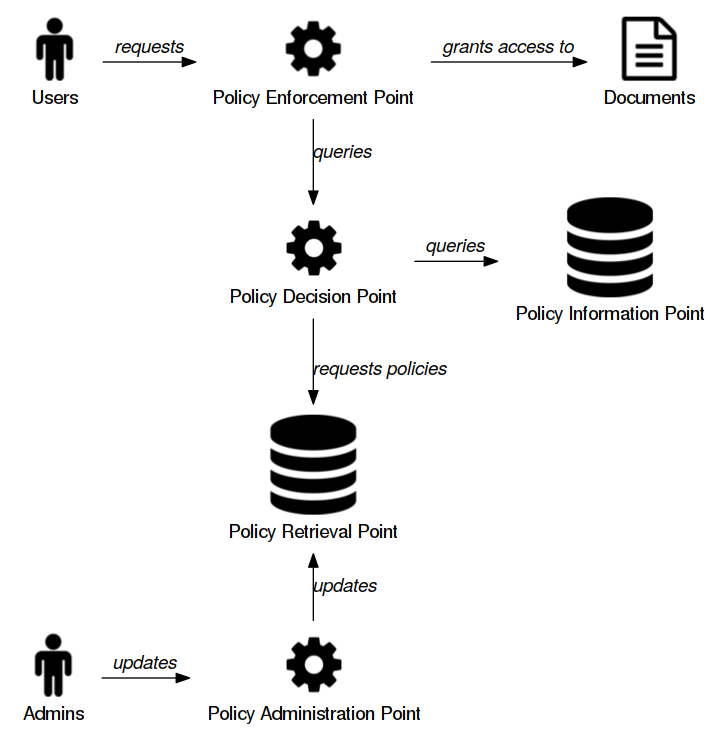
\includegraphics[width=0.6\textwidth]{figures/xacml-architecture.png}
  \caption{The XACML reference architecture.}
  \label{fig:xacml-architecture}
\end{figure}

XACML also defines a reference architecture for anyone using XACML, shown in
\autoref{fig:xacml-architecture}. The architecture consists of five major
\emph{policy points}. The reference architecture describes how to setup the
policy points so that queries can be made and answered automatically. The PEP
stands between the users and the files (for example) they are trying to access.
When a user tries to access a file the PEP sends a query to the PDP (which makes
the \emph{decision}), and \emph{enforces} the policy by either granting or
denying access. In order to make the decision PDP \emph{requests} policies from
the PRP (which are updated by an \emph{administrator} editing the policies at
the PAP), and using \emph{information} from the PIP.

XACML's architecture fits well with a centralized architecture, where
distributed PEPs talk to local PDPs which retrieve policies from a centralized
PRP. For a decentralized scenario the architecture fits less well as the
decision point may have to retrieve policies and decisions from multiple sources
(which may in turn require more decisions and policies to be retrieved).

%Ultimately we chose to use SecPAL as the basis for our work instead of XACML as
%it had well-defined semantics, and was a better fit to describe the
%decentralized policies of the mobile ecosystem. A lot of the results of our work
%could be replicated in XACML instead of AppPAL. 


\section{Fine-Grained Permission Systems}
\label{sec:fine-grained-permissions}

Whilst policy languages, in general, give us a mechanism to describe trust
relationships and decisions \emph{in general}. Fine-grained permission
systems are a type of policy language to control app behavior on
Android. In this section we survey some of the developments here.

This section looks exclusively at Android as that is where the bulk of
the research has been. It is relevant to our work as these alternative
permissions schemes have been used to describe the policies about how
users wish to use their devices. The majority of the work has looked
at Android: perhaps because, unlike iOS, the operating system can be
modified to incorporate new features.

To access some APIs, such as access to private storage, Android apps
must ask for a permission. Permissions are a coarse usage control
mechanism. Until 2015 (and Android Marshmallow), users could not
control which permissions an app had (by default) and not installing
an app was the only way to stop an app accessing data, without
modifying Android.  Since Android Marshmallow, users can disable many
of an app's permissions after installation.

The coarseness of Android's permission system, and its relative
inflexibility, has led to a line of research into \emph{fine-grained}
permissions systems.  These systems add extra permissions controls,
and allow greater control of their enforcement. We describe several
notable examples and what extra controls or new enforcement means the
fine-grained permissions systems offered.  A fine-grained permissions
system is designed to enforce app policies, whereas our work on AppPAL
is about capturing the broader policies of the entire mobile
ecosystem.  A fine-grained permissions system could be \emph{plugged
into} AppPAL, via the constraints mechanisms, to allow enforcement of
fine-grained permissions policies, if we wished to capture and use
these tools.

Some of the earliest work on fine-grained permissions systems for
Android starts with Enck~\etal's work on
Kirin~\cite{enck_lightweight_2009}.  Kirin allowed a user to define
what behavior they considered acceptable using a policy language.
Kirin ran on the device to certify apps using static analysis.  If an
app did not conform to the policy the user would be warned and could
uninstall it.  A natural next question is rather than rejecting the
entire app, can you just reject the behavior you don't like?
Ontang~\etal's SAINT tool~\cite{ongtang_semantically_2012} did just
that for inter-app communication, allowing the user to express a
policy about the circumstances two apps could share data or call
functionality.  Similarly, Apex~\cite{nauman_apex:_2010} allowed
user's to specify at install time constraints as to when a permission
could be used.  CRePE~\cite{conti_crepe:_2010} took these ideas
further allowing permissions to be denied based on \emph{context} (for
example the user was on a train, or the user was within Bluetooth
range of their computer).

Dr{.}~Android and Mr{.}~Hide~\cite{jeon_dr._2012} was a fine-grained
permission scheme that worked by rewriting apps to use guarded APIs.
AppGuard~\cite{backes_appguard_2013} worked similarly to
Dr{.}~Android, but allowed for controlled responses when a permission
was denied---essentially ensuring that the app didn't crash if it
didn't get access to the data it expected
to. Aurasium~\cite{xu_aurasium:_2012} works by modifying apps to
monitor system calls and IPC mechanisms via GOT hijacking in the
Bionic libc, allowing their policies to effect native code which
earlier tools ignored.

Jin~\etal{} developed a fine-grained permission system that targeted
apps written using the PhoneGap framework, that enable developers to
create portable native apps from web
apps~\cite{jin_fine-grained_2015}. Dai~\etal{} proposed a fine-grained
permissions scheme that controlled apps (and IoT devices) access to
media stored on cloud based services based on a user's
policies~\cite{dai_who_2017}.

\section{Moving Forward}

This chapter described SecPAL, and a number of other policy languages designed
in the same time frame. We also described a number of fine-grained permissions
systems that have been used to enforce policies on Android. In the next chapter
we show how we took SecPAL and instantiated it to describe the policies
surrounding mobile devices. In doing so we created AppPAL. We describe the
language and our implementation of it in \autoref{chap:apppal}.

AppPAL fits into this background of policy languages by instantiating SecPAL
for a new domain. It does not have new semantic language features to describe
new kinds of policies.  Instead, its novelty lies in the application to a
domain that has not before had its policies captured using a precise language.

\end{document}

%%% Local Variables:
%%% mode: latex
%%% TeX-master: "../ch2"
%%% End:
